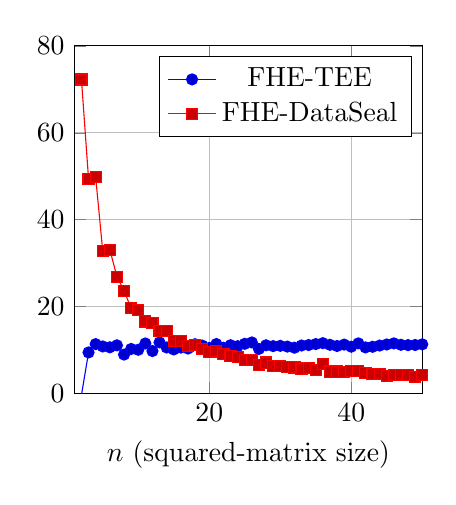
\begin{tikzpicture}
\begin{axis}[
    width=6cm, % Set the width of the plot to the text width of the subfigure
    height=6cm, % You can adjust the height as needed
    xlabel={$n$ (squared-matrix size)},
    % ylabel={Time in Seconds},
    legend pos=north east,
    grid=both,
    xmin=1, xmax=50,
    ymin=0, ymax=80
]
\addplot table {
n	FHE-TEE
2	-0.29
3	9.49
4	11.40
5	10.87
6	10.67
7	11.12
8	9.00
9	10.29
10	10.10
11	11.55
12	9.81
13	11.80
14	10.63
15	10.18
16	10.61
17	10.39
18	11.38
19	11.07
20	10.53
21	11.42
22	10.56
23	11.15
24	10.93
25	11.47
26	11.79
27	10.30
28	11.13
29	10.94
30	11.01
31	10.83
32	10.58
33	11.08
34	11.19
35	11.41
36	11.62
37	11.24
38	10.97
39	11.29
40	10.81
41	11.57
42	10.65
43	10.79
44	11.07
45	11.32
46	11.57
47	11.24
48	11.17
49	11.20
50	11.35
};
\addlegendentry{FHE-TEE}

\addplot table {
n	vFHE
2	72.25
3	49.38
4	49.83
5	32.79
6	33.10
7	26.90
8	23.69
9	19.62
10	19.32
11	16.61
12	16.30
13	14.37
14	14.38
15	12.21
16	12.13
17	10.99
18	11.11
19	10.27
20	9.68
21	9.72
22	9.05
23	8.64
24	8.47
25	7.79
26	7.72
27	6.65
28	7.16
29	6.38
30	6.42
31	6.16
32	6.03
33	5.79
34	5.97
35	5.40
36	6.76
37	5.09
38	5.09
39	4.99
40	5.18
41	5.19
42	4.69
43	4.51
44	4.52
45	4.08
46	4.25
47	4.38
48	4.23
49	3.91
50	4.26
};
\addlegendentry{FHE-DataSeal}

\end{axis}
\end{tikzpicture}